\begin{document}
	\subsection{Healty Control}
	
	In this subsection I will discuss the results of the segmentation made on $8$ healthy controls scans. This kind of  test was performed as benchmark, in order to ensure that, in absence of lesion, no areas were detected. On the other hand, this kind of segmentation is useful since allows to find the main sources of misclassified areas, which we will see are represented by motion artifacts
	
	\begin{figure}[h!]
		\centering
			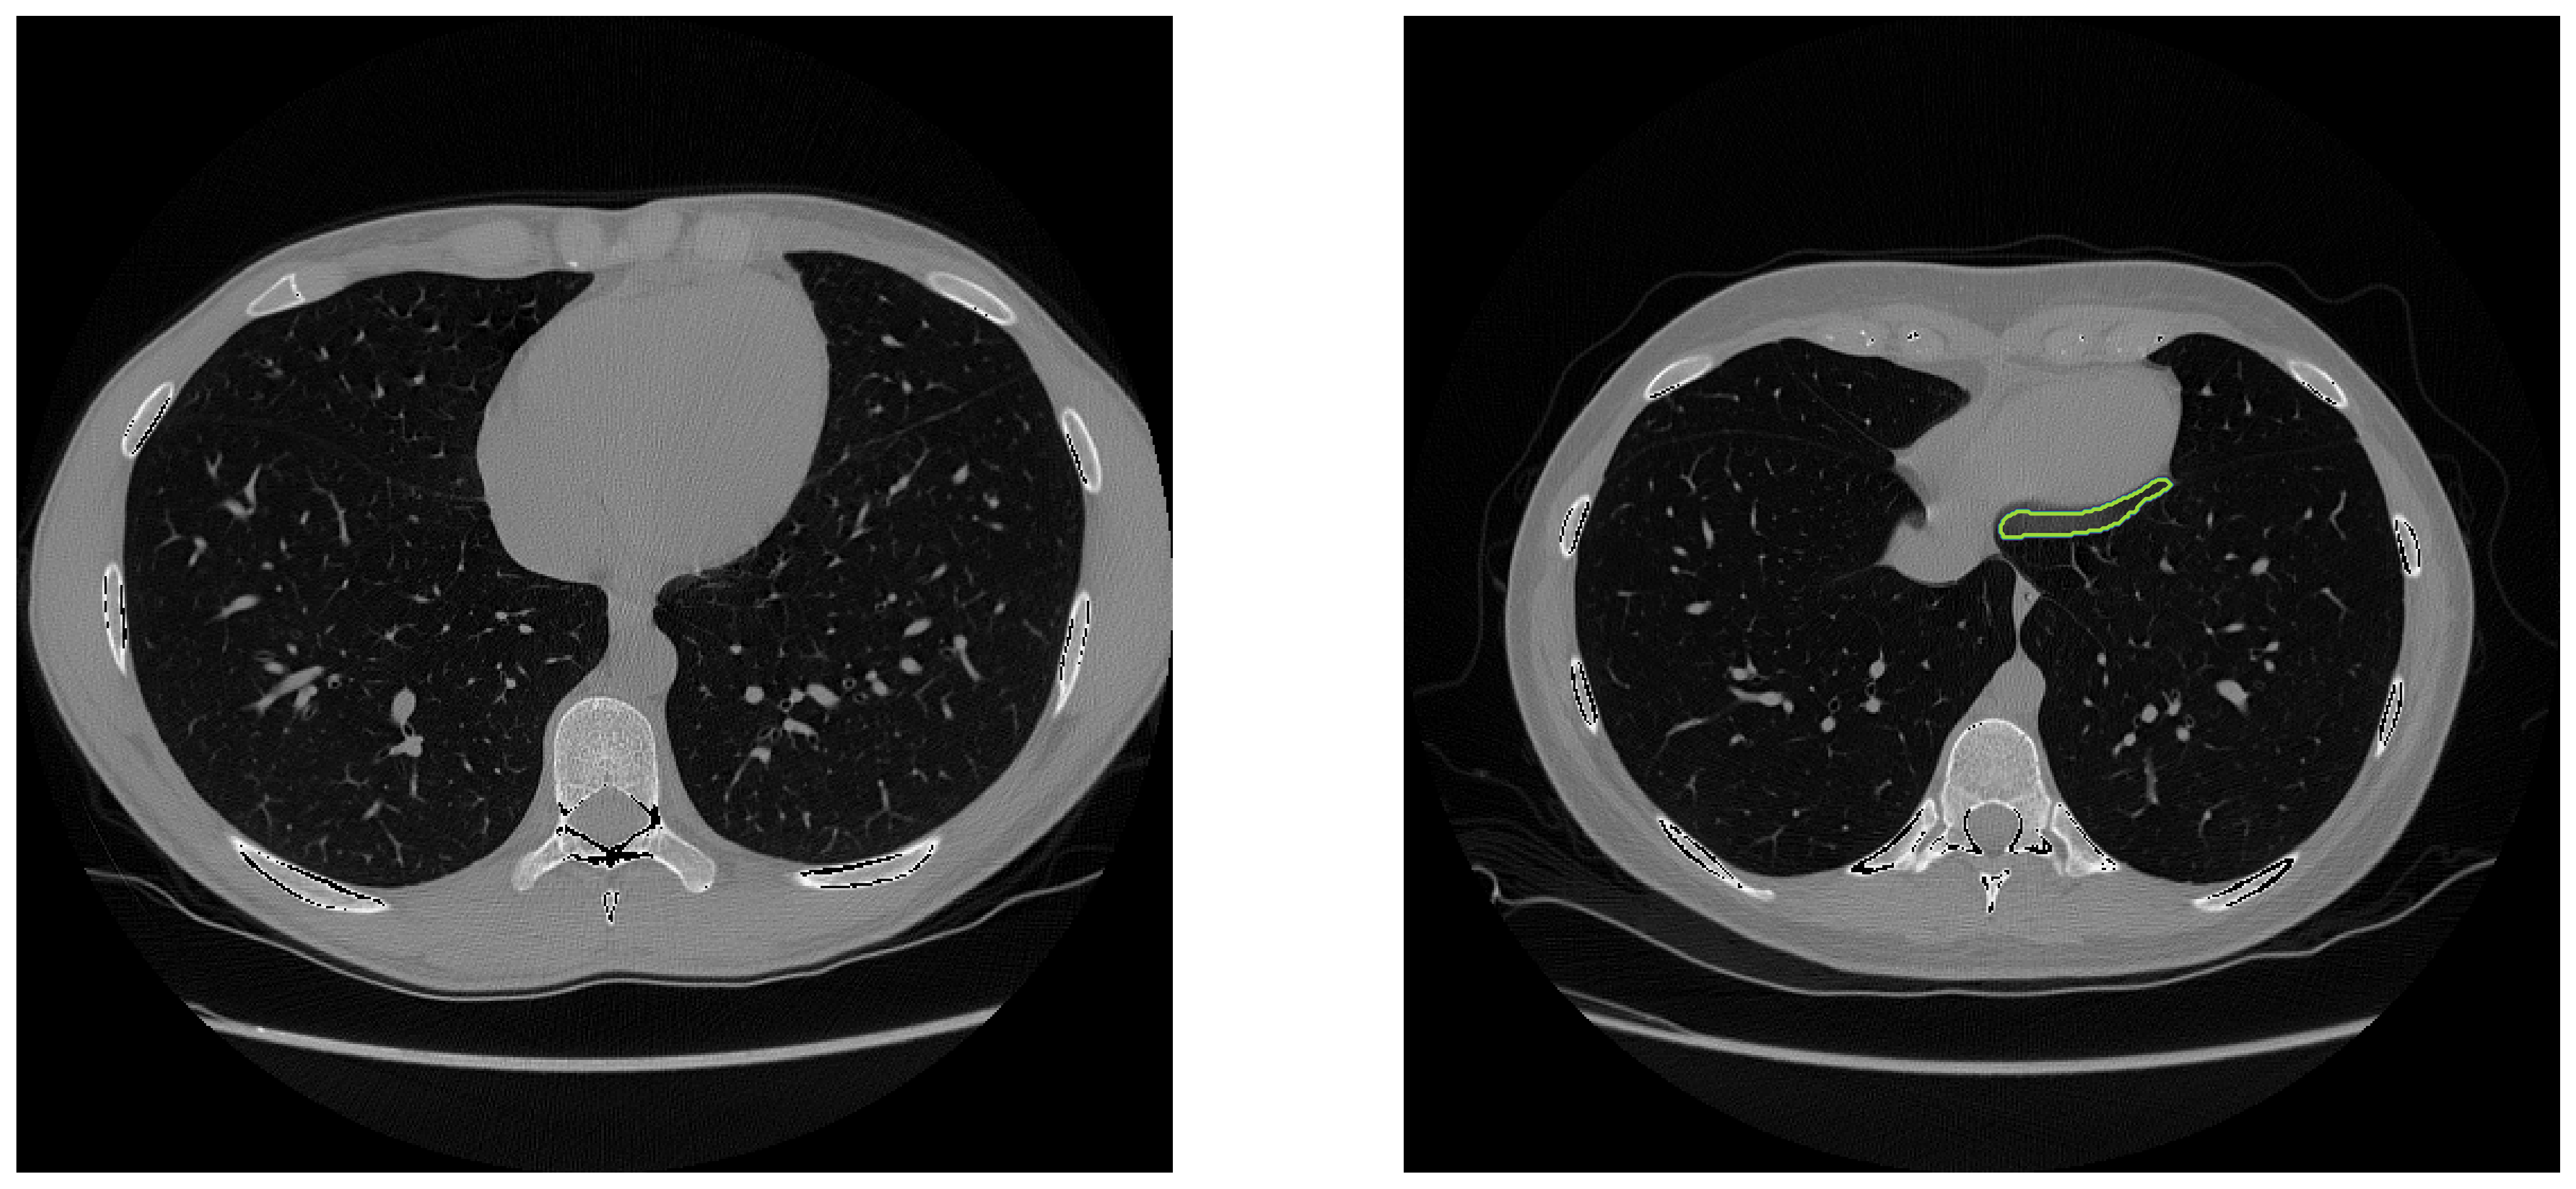
\includegraphics[scale=.4]{HeathyConrol.png}
			\caption{Segmented CT scans from healthy controls: Without motion artifacts(left), with motion artifacts(right). In the first case we can see that no area is identified since no lesion is present; In second one we can see how, in presence of motion artifacts, some false positives may raise.  }\label{fig:HealthyControl}
	\end{figure}

	In \figurename\,\ref{fig:HealthyControl} I have displayed two segmented scans from healthy control. We can see that, in a normal case, no lesion areas were detected; but in presence of artifacts, some misclassified regions appears.
	
	This result suggests that the main source of false positives is the presence of motion artifacts, caused by heartbeat and respiratory cycle.
	
	In the end we have verified that, in the most common case, no lesion areas were identified as we expect. On the other hand, in presence of motion artifacts, these may be misclassified as lesions and we have observed that this is one of the main source of false positives. 
	
	
	

\end{document}